%\setchapterimage{bandeau}
\chapter*{TD \arabic{cptTD} \\ 
Contrôle d'une machine de forage -- 
\ifprof Corrigé \else Sujet \fi}
\addcontentsline{toc}{section}{TD \arabic{cptTD} :
Contrôle d'une machine de forage -- 
\ifprof Corrigé \else Sujet \fi}

\iflivret \stepcounter{cptTD} \else
\ifprof  \stepcounter{cptTD} \else \fi
\fi

\setcounter{question}{0}
\marginnote{D'après Concours CCINP 2023 -- MP.}
%\marginnote[1cm]{
%\UPSTIcompetence[2]{C1-02}
%\UPSTIcompetence[2]{C2-04}}





On travaille avec le schéma-bloc simplifié de la figure \ref{Cy_02_Ch_04_TD_03_fig_12} où $K_0$ est un gain d’adaptation fixe. 


\begin{figure}[!h]
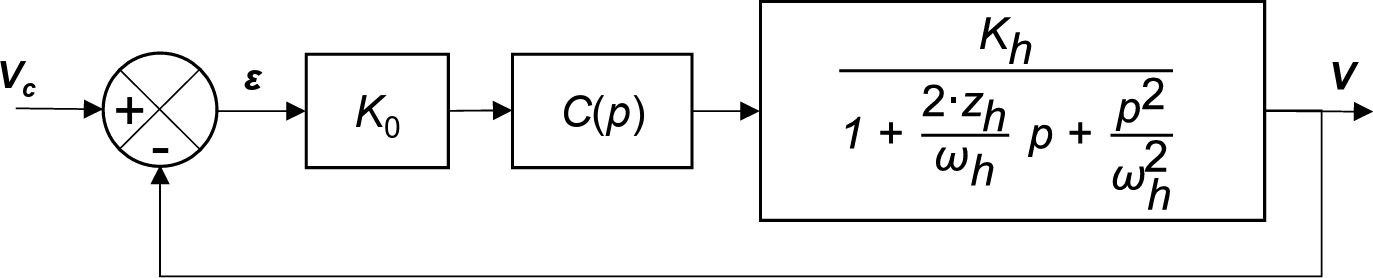
\includegraphics[width=.7\linewidth]{fig_12}
\caption{Schéma-bloc de l’asservissement en vitesse simplifié \label{Cy_02_Ch_04_TD_03_fig_12}}
\end{figure}

 On prend dans un premier temps un correcteur $C(p)$ proportionnel : $C(p) = K_p$. 
 
%Q 25
\question{Exprimer la fonction de transfert en boucle ouverte $\indice{G}{BO}(p)=\dfrac{V(p)}{\varepsilon(p)}$.}
\ifprof
\begin{corrige}
\end{corrige}
\else
\fi


\begin{marginfigure}
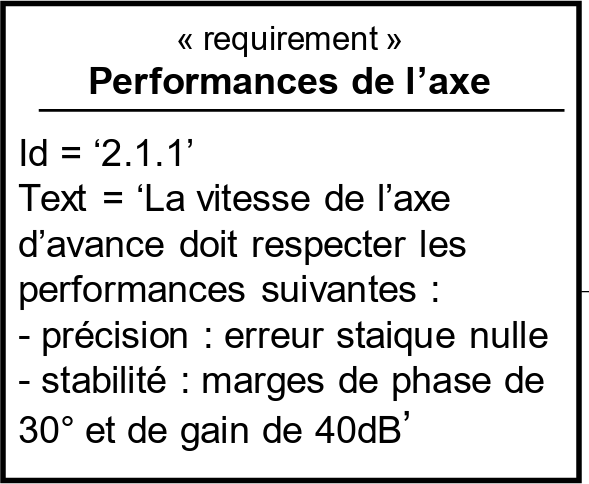
\includegraphics[width=\linewidth]{req}
%\caption{ Schéma-bloc de l’asservissement en vitesse simplifié \label{Cy_02_Ch_04_TD_03_fig_12}}
\end{marginfigure}

%Q26. 
\question{Avec un correcteur proportionnel, peut-on satisfaire l’exigence de précision de vitesse 
indiquée à l’exigence 2.1.1. ? Justifier.}
\ifprof
\begin{corrige}
\end{corrige}
\else
\fi

 
On utilise dans un second temps un correcteur proportionnel intégral : $C(p)=K_P\left( 1+\dfrac{1}{T_i p}\right)$.
 
%Q27. 
\question{L’exigence de précision sur la vitesse est-elle satisfaite ? Justifier. }
\ifprof
\begin{corrige}
\end{corrige}
\else
\fi

 Ce correcteur est initialement réglé avec les valeurs suivantes : $K_p = 1$ et $T_i = \SI{10}{s}$. 
 
%Q28. 
\question{Tracer les diagrammes de Bode asymptotique et réel de ce correcteur. Détailler 
les constructions. }
\ifprof
\begin{corrige}
\end{corrige}
\else
\fi

\begin{figure}[!h]
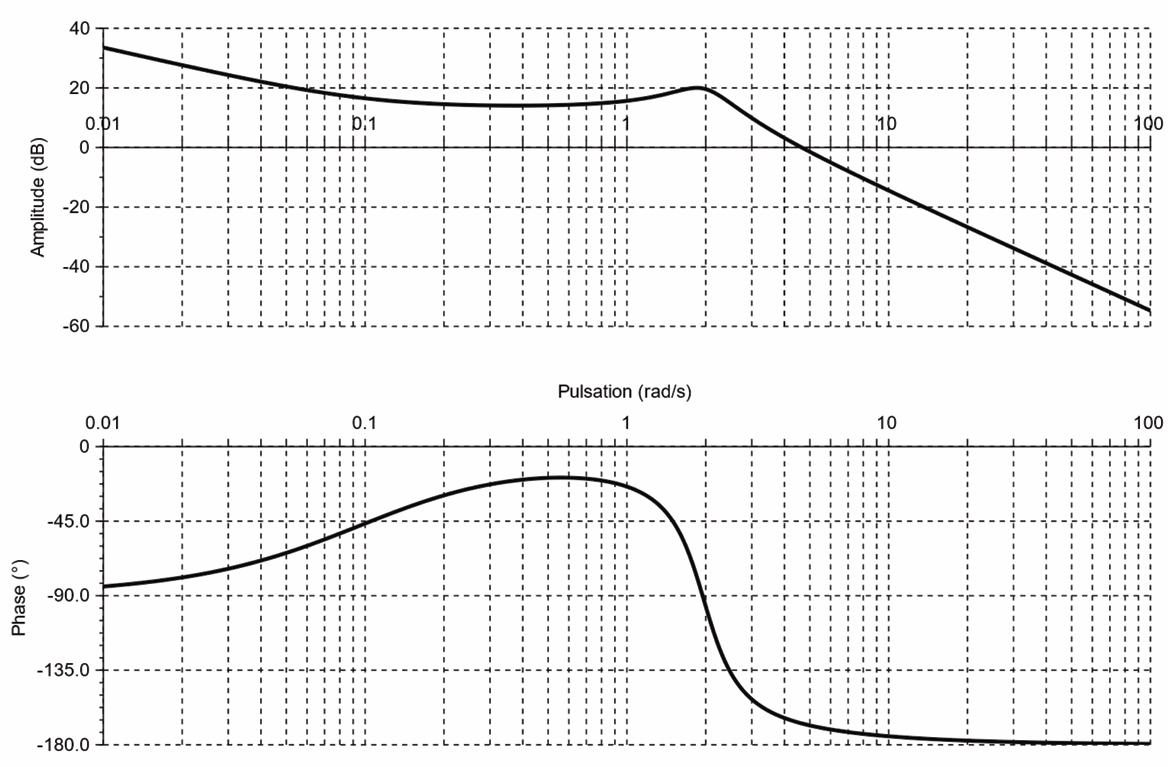
\includegraphics[width=\linewidth]{dr_03}
%\caption{ Schéma-bloc de l’asservissement en vitesse simplifié \label{Cy_02_Ch_04_TD_03_fig_12}}
\end{figure}

 
Pour le réglage de la question précédente, on donne le diagramme de Bode de la fonction de 
transfert en boucle ouverte ainsi corrigée sur le DR3. 

% Q29. 
\question{Affiner le réglage du correcteur (sans modifier la valeur de $T_i$) en proposant une valeur de $K_p$ permettant de garantir la marge de phase spécifiée dans l’exigence 2.1.1. On répondra à cette 
question sur la figure précente.}
\ifprof
\begin{corrige}
\end{corrige}
\else
\fi
 
 
Enfin, on souhaite valider ou invalider l’hypothèse faite en début de cette sous-partie concernant la 
non-influence de l’amortisseur sur les performances d’asservissement en vitesse d’avance de la 
table de forage. Les diagrammes de Bode de la figure suivante, 
illustrent la fonction de transfert en boucle ouverte corrigée sans (en train plein) et avec amortisseur 
(en pointillés). 
 
 
\begin{figure}[!h]
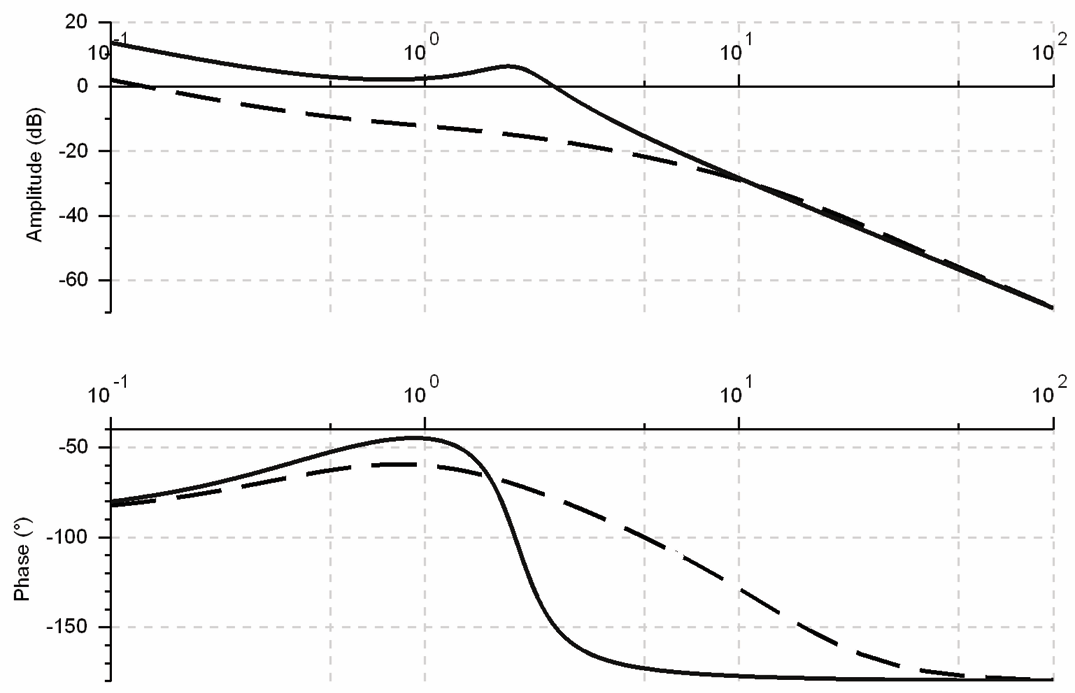
\includegraphics[width=\linewidth]{dr_04}
%\caption{ Schéma-bloc de l’asservissement en vitesse simplifié \label{Cy_02_Ch_04_TD_03_fig_12}}
\end{figure}

 
%Q30. 
\question{Sur quelle(s) performance(s) la présence de l’amortisseur peut-elle influer ? Justifier que le correcteur choisi permet de répondre aux exigences 2.1.1 en présence de l'amortisseur.}
\ifprof
\begin{corrige}
\end{corrige}
\else
\fi




